\section{The Consumer}

\subsection{Register}
\textbf{Pre-conditions}: The consumer does not have an existing
customer profile.\\

\textbf{Post-conditions}: A new customer profile exists in the
system, with a name, email and password and the consumer is logged
in.\\

\textbf{Purpose}: The consumer wants to book tickets for an
upcoming show.\\

\textbf{Description}: The consumer fills in a registration form with
their desired name, email and password. Once complete, they press
the register button and they will be automatically logged in after
their customer profile has been created on the system.

\subsection{Login}
\textbf{Pre-conditions}: The consumer has a customer profile.\\

\textbf{Post-conditions}: The consumer is logged in.\\

\textbf{Purpose}: The consumer has previously bought tickets for a
show and wants to buy tickets for an upcoming show.\\

\textbf{Description}: The consumer enters their email and password.
The details are verified on the system and if they are valid, the
user is logged in. If the credentials are invalid, the consumer is
prompted to re-enter their email and password.

\subsection{Update User Profile}
\textbf{Pre-conditions}: The consumer has a customer profile and is
logged in.\\

\textbf{Post-conditions}: The stored customer profile information is
modified.\\

\textbf{Purpose}: The consumer wants to change their email, shipping
address or password.\\

\textbf{Description}: The consumer updates the fields they wish to
change (e.g, their shipping address). Once they are happy with the
changes, they click the save button and their customer profile will
be modified on the system.

\subsection{View Upcoming Events}
\textbf{Pre-conditions}: Zero or more events exists.\\

\textbf{Purpose}: The consumer wants to see all the upcoming events
that they can book tickets for.\\

\textbf{Description}: The consumer is presented with a list of
events. Selecting an event will show the list of shows assigned to
the event. If there are no upcoming events, then the list will be
empty with a message indicating there are no events on.

\subsection{View Shows by Date}
\textbf{Pre-conditions}: Zero or more shows exist.\\

\textbf{Purpose}: The consumer wants to see all the shows on over a
range of days.\\

\textbf{Description}: The consumer is presented with a list of shows
that are taking place within their specified date range. Selecting
a show will allow the consumer to book tickets for the show. If
there are no shows taking place in this date range, the list will be
empty with a message indicating there are no shows.

\subsection{Purchase Tickets}
\textbf{Pre-conditions}: The consumer is logged in and one or more
shows exist.\\

\textbf{Post-conditions}: A new ticket exists in the system.\\

\textbf{Purpose}: The consumer wants to buy one or more tickets for
a selected show.\\

\textbf{Description}: The consumer is asked how many tickets they
wish to purchase. After selecting the amount, the system displays
the best available seat(s) with their price. The consumer also has
the option of manually picking their seats via a button. The manual
option displays a seating chart with the available seats
highlighted. The consumer can then select the needed amount of
seats. With both methods, the currently selected seats are reserved
and not available to other consumers that are booking tickets for
the same show. The reservation is cancelled once the transaction
is cancelled or has not been completed after 5 minutes.\\

Once they are happy with the selected seats, the consumer is
shown the total cost of the tickets. Here they are able to add a
valid promotion for the show. The consumer can then enter their
credit card information and confirm the purchase.\\

Upon confirmation of the purchase, the ticket(s) are added to the
system and displayed again to the user as a receipt.

\subsection{View Tickets}
\textbf{Pre-conditions}: The consumer is logged in.\\

\textbf{Purpose}: The consumer wants to see their past purchases.\\

\textbf{Description}: The consumer is presented with a list of
their tickets, showing the price, date and seat number.

\subsection{Diagrams}

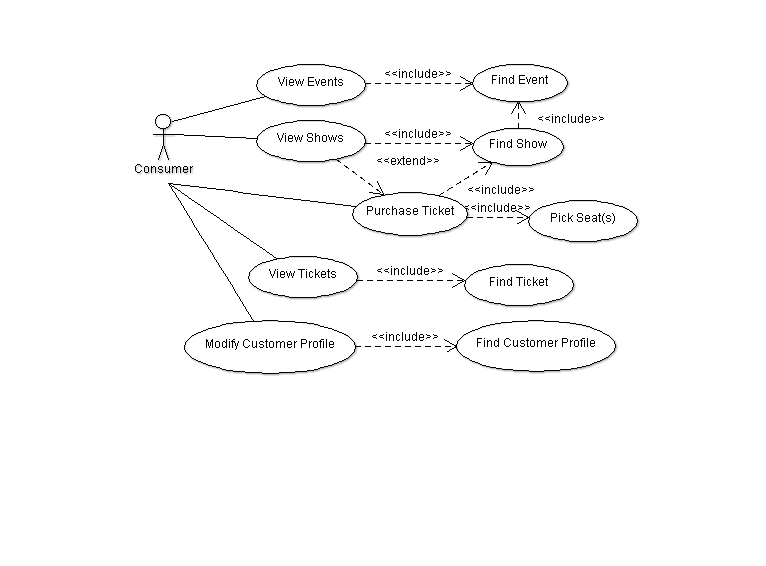
\includegraphics[width=\linewidth]{ConsumerUsecaseDiagram}
